\documentclass{article}

\usepackage{graphicx}
\usepackage{hyperref}
\begin{document}
\begin{titlepage}
\begin{center} 
\line(1,0){300}\\
[0.25in]
\huge{\bfseries REPORT}\\
[2mm]
\line(1,0){200}\\
[.5cm]
\textsc{\LARGE DISCRETE MATHEMATICS}\\
[5cm]
\end{center}
\begin{flushright}
\textsc{\Large Rabita Islam Satue\\}
Sheikh Hasina Institute of ICT\\
Bangabondhu Sheikh Mujibur Rahman\\ Science and Technology University\\
ID:18ICTCSE012\\
Email:rabitaislamsatue2682@gmail.com\\
29 November,2019
\end{flushright}
\end{titlepage}
\tableofcontents
\thispagestyle{empty}
\cleardoublepage
\setcounter{page}{1}
\section{Introduction}\label{sec:intro}

Discrete mathematics is the study of mathematical structures that are fundamentally discrete rather than continuous. In contrast to real numbers that have the property of varying "smoothly", the objects studied in discrete mathematics – such as integers, graphs, and statements in logic – do not vary smoothly in this way, but have distinct, separated values.Discrete mathematics therefore excludes topics in "continuous mathematics" such as calculus or Euclidean geometry. Discrete objects can often be enumerated by integers. More formally, discrete mathematics has been characterized as the branch of mathematics dealing with countable sets (finite sets or sets with the same cardinality as the natural numbers). However, there is no exact definition of the term "discrete mathematics." Indeed, discrete mathematics is described less by what is included than by what is excluded: continuously varying quantities and related notions.

The set of objects studied in discrete mathematics can be finite or infinite. The term finite mathematics is sometimes applied to parts of the field of discrete mathematics that deals with finite sets, particularly those areas relevant to business.

Research in discrete mathematics increased in the latter half of the twentieth century partly due to the development of digital computers which operate in discrete steps and store data in discrete bits. Concepts and notations from discrete mathematics are useful in studying and describing objects and problems in branches of computer science, such as computer algorithms, programming languages, cryptography, automated theorem proving, and software development. Conversely, computer implementations are significant in applying ideas from discrete mathematics to real-world problems, such as in operations research.

Although the main objects of study in discrete mathematics are discrete objects, analytic methods from continuous mathematics are often employed as well.

In university curricula, "Discrete Mathematics" appeared in the 1980s, initially as a computer science support course; its contents were somewhat haphazard at the time. The curriculum has thereafter developed in conjunction with efforts by ACM and MAA into a course that is basically intended to develop mathematical maturity in first-year students; therefore it is nowadays a prerequisite for mathematics majors in some universities as well.[6][7] Some high-school-level discrete mathematics textbooks have appeared as well.[8] At this level, discrete mathematics is sometimes seen as a preparatory course, not unlike precalculus in this respect.
\begin{figure}[h]
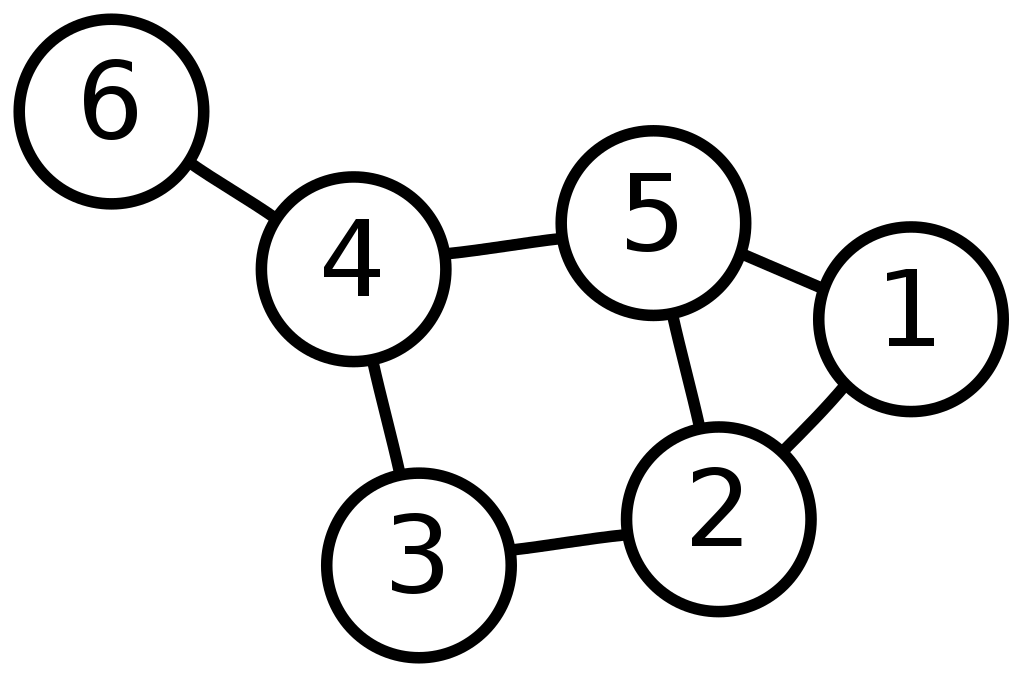
\includegraphics[width=0.4\textwidth]{sa.png}
\caption{}
\end{figure}
\newpage
\section{History}
The term "Discrete Mathematics" is probably best defined as the areas of math, that don't deal with real numbers - it deals with a variety of areas in which the the values are not continuous, such as integers or logic.

The usual sequence of math in high school and college mainly was a calculus sequence. As computers became more important, and because computers work with binary numbers and computer instructions are not executed continuously (meaning that they are executed one instruction at a time) discrete math topics became more important.

So in a sense discrete mathematics encompasses a variety of areas, not neccessary related, that are important in computer science, and later, many other fields.

At the university level, books on discrete mathematics started coming out around 1980, and since then the topics covered have been somewhat standardized.

Here are just some of the topics covered:

- logic
- set theory
- functions
- recursion
- proofs
- number theory
- combinatorics (counting)
- graph theory
- tree theory
- finite state machines
- cryptography
- the theory of computatios.
\section{Grand challenges, past and present}
The history of discrete mathematics has involved a number of challenging problems which have focused attention within areas of the field. In graph theory, much research was motivated by attempts to prove the four color theorem, first stated in 1852, but not proved until 1976 (by Kenneth Appel and Wolfgang Haken, using substantial computer assistance).

In logic, the second problem on David Hilbert's list of open problems presented in 1900 was to prove that the axioms of arithmetic are consistent. Gödel's second incompleteness theorem, proved in 1931, showed that this was not possible – at least not within arithmetic itself. Hilbert's tenth problem was to determine whether a given polynomial Diophantine equation with integer coefficients has an integer solution. In 1970, Yuri Matiyasevich proved that this could not be done.

The need to break German codes in World War II led to advances in cryptography and theoretical computer science, with the first programmable digital electronic computer being developed at England's Bletchley Park with the guidance of Alan Turing and his seminal work, On Computable Numbers.At the same time, military requirements motivated advances in operations research. The Cold War meant that cryptography remained important, with fundamental advances such as public-key cryptography being developed in the following decades. Operations research remained important as a tool in business and project management, with the critical path method being developed in the 1950s. The telecommunication industry has also motivated advances in discrete mathematics, particularly in graph theory and information theory. Formal verification of statements in logic has been necessary for software development of safety-critical systems, and advances in automated theorem proving have been driven by this need.

Computational geometry has been an important part of the computer graphics incorporated into modern video games and computer-aided design tools.

Several fields of discrete mathematics, particularly theoretical computer science, graph theory, and combinatorics, are important in addressing the challenging bioinformatics problems associated with understanding the tree of life.

Currently, one of the most famous open problems in theoretical computer science is the P = NP problem, which involves the relationship between the complexity classes P and NP. The Clay Mathematics Institute has offered a million USD prize for the first correct proof, along with prizes for six other mathematical problems.
Graphs like this are among the objects studied by discrete mathematics, for their interesting mathematical properties, their usefulness as models of real-world problems, and their importance in developing computer algorithms.
\begin{figure}[h]
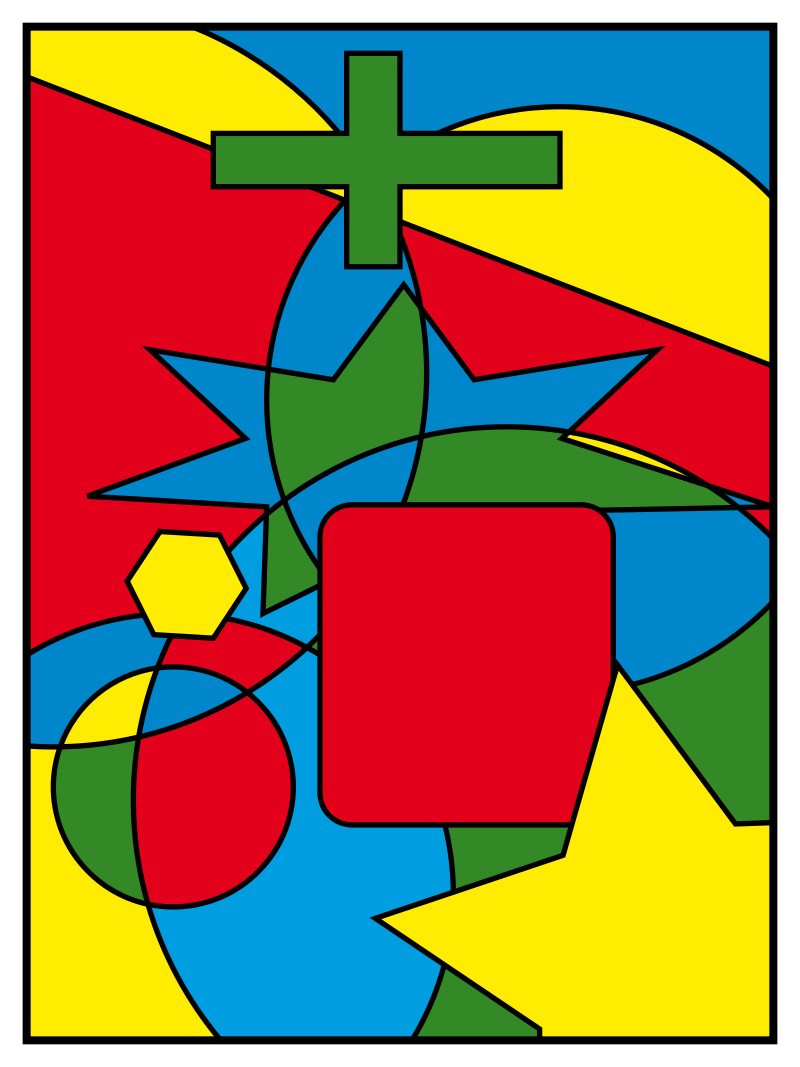
\includegraphics[width=0.3\textwidth]{sb.png}
\caption{Grand Challenge}
\end{figure}
\newpage
\section{Topics in discrete mathematics}
\subsection{Theoretical computer science}
Theoretical computer science includes areas of discrete mathematics relevant to computing. It draws heavily on graph theory and mathematical logic. Included within theoretical computer science is the study of algorithms and data structures. Computability studies what can be computed in principle, and has close ties to logic, while complexity studies the time, space, and other resources taken by computations. Automata theory and formal language theory are closely related to computability. Petri nets and process algebras are used to model computer systems, and methods from discrete mathematics are used in analyzing VLSI electronic circuits. Computational geometry applies algorithms to geometrical problems, while computer image analysis applies them to representations of images. Theoretical computer science also includes the study of various continuous computational topics. 
\subsection{Information theory}
Information theory involves the quantification of information. Closely related is coding theory which is used to design efficient and reliable data transmission and storage methods. Information theory also includes continuous topics such as: analog signals, analog coding, analog encryption.
\subsection{Logic}
Logic is the study of the principles of valid reasoning and inference, as well as of consistency, soundness, and completeness. For example, in most systems of logic (but not in intuitionistic logic) Peirce's law (((P→Q)→P)→P) is a theorem. For classical logic, it can be easily verified with a truth table. The study of mathematical proof is particularly important in logic, and has applications to automated theorem proving and formal verification of software.

Logical formulas are discrete structures, as are proofs, which form finite trees[14] or, more generally, directed acyclic graph structures[15][16] (with each inference step combining one or more premise branches to give a single conclusion). The truth values of logical formulas usually form a finite set, generally restricted to two values: true and false, but logic can also be continuous-valued, e.g., fuzzy logic. Concepts such as infinite proof trees or infinite derivation trees have also been studied.
\begin{figure}[h]
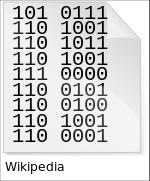
\includegraphics[width=0.4\textwidth]{sc.png}
\caption{Logic}
\end{figure}
\subsection{Set theory} 
Set theory is the branch of mathematics that studies sets, which are collections of objects, such as {blue, white, red} or the (infinite) set of all prime numbers. Partially ordered sets and sets with other relations have applications in several areas.

In discrete mathematics, countable sets (including finite sets) are the main focus. The beginning of set theory as a branch of mathematics is usually marked by Georg Cantor's work distinguishing between different kinds of infinite set, motivated by the study of trigonometric series, and further development of the theory of infinite sets is outside the scope of discrete mathematics. Indeed, contemporary work in descriptive set theory makes extensive use of traditional continuous mathematics. 
\begin{figure}[h]
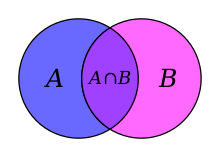
\includegraphics[width=0.4\textwidth]{sg.png}
\caption{set thory}
\end{figure}
\newpage
\subsubsection{History}
Mathematical topics typically emerge and evolve through interactions among many researchers. Set theory, however, was founded by a single paper in 1874 by Georg Cantor: "On a Property of the Collection of All Real Algebraic Numbers".[2][3]

Since the 5th century BC, beginning with Greek mathematician Zeno of Elea in the West and early Indian mathematicians in the East, mathematicians had struggled with the concept of infinity. Especially notable is the work of Bernard Bolzano in the first half of the 19th century.[4] Modern understanding of infinity began in 1870–1874 and was motivated by Cantor's work in real analysis.[5] An 1872 meeting between Cantor and Richard Dedekind influenced Cantor's thinking and culminated in Cantor's 1874 paper.

Cantor's work initially polarized the mathematicians of his day. While Karl Weierstrass and Dedekind supported Cantor, Leopold Kronecker, now seen as a founder of mathematical constructivism, did not. Cantorian set theory eventually became widespread, due to the utility of Cantorian concepts, such as one-to-one correspondence among sets, his proof that there are more real numbers than integers, and the "infinity of infinities" ("Cantor's paradise") resulting from the power set operation. This utility of set theory led to the article "Mengenlehre" contributed in 1898 by Arthur Schoenflies to Klein's encyclopedia.

The next wave of excitement in set theory came around 1900, when it was discovered that some interpretations of Cantorian set theory gave rise to several contradictions, called antinomies or paradoxes. Bertrand Russell and Ernst Zermelo independently found the simplest and best known paradox, now called Russell's paradox: consider "the set of all sets that are not members of themselves", which leads to a contradiction since it must be a member of itself and not a member of itself. In 1899 Cantor had himself posed the question "What is the cardinal number of the set of all sets?", and obtained a related paradox. Russell used his paradox as a theme in his 1903 review of continental mathematics in his The Principles of Mathematics.

In 1906 English readers gained the book Theory of Sets of Points[6] by husband and wife William Henry Young and Grace Chisholm Young, published by Cambridge University Press.

The momentum of set theory was such that debate on the paradoxes did not lead to its abandonment. The work of Zermelo in 1908 and the work of Abraham Fraenkel and Thoralf Skolem in 1922 resulted in the set of axioms ZFC, which became the most commonly used set of axioms for set theory. The work of analysts such as Henri Lebesgue demonstrated the great mathematical utility of set theory, which has since become woven into the fabric of modern mathematics. Set theory is commonly used as a foundational system, although in some areas—such as algebraic geometry and algebraic topology—category theory is thought to be a preferred foundation. 
\begin{figure}[h]
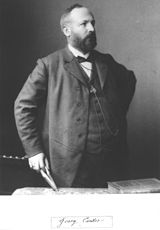
\includegraphics[width=0.4\textwidth]{sh.jpg}
\caption{Georg Cantor}
\end{figure}
\subsubsection{Basic concepts and notation}
Set theory begins with a fundamental binary relation between an object o and a set A. If o is a member (or element) of A, the notation o ∈ A is used. A set is described by listing elements separated by commas, or by a characterizing property of its elements, within braces { }. Since sets are objects, the membership relation can relate sets as well.

A derived binary relation between two sets is the subset relation, also called set inclusion. If all the members of set A are also members of set B, then A is a subset of B, denoted A ⊆ B. For example, {1, 2} is a subset of {1, 2, 3} , and so is {2} but {1, 4} is not. As insinuated from this definition, a set is a subset of itself. For cases where this possibility is unsuitable or would make sense to be rejected, the term proper subset is defined. A is called a proper subset of B if and only if A is a subset of B, but A is not equal to B. Also 1, 2, and 3 are members (elements) of the set {1, 2, 3} but are not subsets of it; and in turn, the subsets, such as {1}, are not members of the set {1, 2, 3}.

Just as arithmetic features binary operations on numbers, set theory features binary operations on sets.[7] The:

    Union of the sets A and B, denoted A ∪ B, is the set of all objects that are a member of A, or B, or both. The union of {1, 2, 3} and {2, 3, 4} is the set {1, 2, 3, 4} .
    Intersection of the sets A and B, denoted A ∩ B, is the set of all objects that are members of both A and B. The intersection of {1, 2, 3} and {2, 3, 4} is the set {2, 3} .
    Set difference of U and A, denoted U \ A, is the set of all members of U that are not members of A. The set difference {1, 2, 3} \ {2, 3, 4} is {1} , while, conversely, the set difference {2, 3, 4} \ {1, 2, 3} is {4} . When A is a subset of U, the set difference U \ A is also called the complement of A in U. In this case, if the choice of U is clear from the context, the notation Ac is sometimes used instead of U \ A, particularly if U is a universal set as in the study of Venn diagrams.
    Symmetric difference of sets A and B, denoted A △ B or A ⊖ B, is the set of all objects that are a member of exactly one of A and B (elements which are in one of the sets, but not in both). For instance, for the sets {1, 2, 3} and {2, 3, 4} , the symmetric difference set is {1, 4} . It is the set difference of the union and the intersection, (A ∪ B) \ (A ∩ B) or (A \ B) ∪ (B \ A).
    Cartesian product of A and B, denoted A × B, is the set whose members are all possible ordered pairs (a, b) where a is a member of A and b is a member of B. The cartesian product of {1, 2} and {red, white} is {(1, red), (1, white), (2, red), (2, white)}.
    Power set of a set A is the set whose members are all of the possible subsets of A. For example, the power set of {1, 2} is { {}, {1}, {2}, {1, 2} } .

Some basic sets of central importance are the empty set (the unique set containing no elements; occasionally called the null set though this name is ambiguous), the set of natural numbers, and the set of real numbers.
\subsubsection{Some ontology}
A set is pure if all of its members are sets, all members of its members are sets, and so on. For example, the set {{}} containing only the empty set is a nonempty pure set. In modern set theory, it is common to restrict attention to the von Neumann universe of pure sets, and many systems of axiomatic set theory are designed to axiomatize the pure sets only. There are many technical advantages to this restriction, and little generality is lost, because essentially all mathematical concepts can be modeled by pure sets. Sets in the von Neumann universe are organized into a cumulative hierarchy, based on how deeply their members, members of members, etc. are nested. Each set in this hierarchy is assigned (by transfinite recursion) an ordinal number α known as its rank. The rank of a pure set X is defined to be the least upper bound of all successors of ranks of members of X. For example, the empty set is assigned rank 0, while the set {{}} containing only the empty set is assigned rank 1. For each ordinal α the set V α V is defined to consist of all pure sets with rank less than α.
\begin{figure}[h]
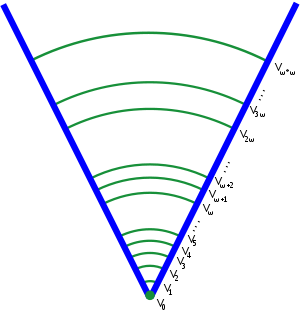
\includegraphics[width=0.4\textwidth]{si.png}
\caption{An initial segment of the von Neumann hierarchy.}
\end{figure}
\subsection{Combinatorics}
Combinatorics studies the way in which discrete structures can be combined or arranged. Enumerative combinatorics concentrates on counting the number of certain combinatorial objects - e.g. the twelvefold way provides a unified framework for counting permutations, combinations and partitions. Analytic combinatorics concerns the enumeration (i.e., determining the number) of combinatorial structures using tools from complex analysis and probability theory. In contrast with enumerative combinatorics which uses explicit combinatorial formula and generating functions to describe the results, analytic combinatorics aims at obtaining asymptotic formula. Design theory is a study of combinatorial designs, which are collections of subsets with certain intersection properties. Partition theory studies various enumeration and asymptotic problems related to integer partitions, and is closely related to q-series, special functions and orthogonal polynomials. Originally a part of number theory and analysis, partition theory is now considered a part of combinatorics or an independent field. Order theory is the study of partially ordered sets, both finite and infinite. 
\subsection{Graph Theory}
Graph theory, the study of graphs and networks, is often considered part of combinatorics, but has grown large enough and distinct enough, with its own kind of problems, to be regarded as a subject in its own right.Graphs are one of the prime objects of study in discrete mathematics. They are among the most ubiquitous models of both natural and human-made structures. They can model many types of relations and process dynamics in physical, biological and social systems. In computer science, they can represent networks of communication, data organization, computational devices, the flow of computation, etc. In mathematics, they are useful in geometry and certain parts of topology, e.g. knot theory. Algebraic graph theory has close links with group theory. There are also continuous graphs; however, for the most part, research in graph theory falls within the domain of discrete mathematics.
\subsection{Probability}
Discrete probability theory deals with events that occur in countable sample spaces. For example, count observations such as the numbers of birds in flocks comprise only natural number values {0, 1, 2, ...}. On the other hand, continuous observations such as the weights of birds comprise real number values and would typically be modeled by a continuous probability distribution such as the normal. Discrete probability distributions can be used to approximate continuous ones and vice versa. For highly constrained situations such as throwing dice or experiments with decks of cards, calculating the probability of events is basically enumerative combinatorics. 
\subsection{Number Theory}
Number theory is concerned with the properties of numbers in general, particularly integers. It has applications to cryptography and cryptanalysis, particularly with regard to modular arithmetic, diophantine equations, linear and quadratic congruences, prime numbers and primality testing. Other discrete aspects of number theory include geometry of numbers. In analytic number theory, techniques from continuous mathematics are also used. Topics that go beyond discrete objects include transcendental numbers, diophantine approximation, p-adic analysis and function fields.
\begin{figure}[h]
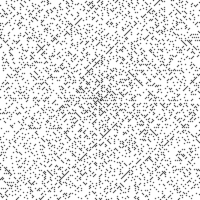
\includegraphics[width=0.4\textwidth]{sd.png}
\caption{Number Theory}
\end{figure}
\newpage
\subsection{Algebra}
Algebraic structures occur as both discrete examples and continuous examples. Discrete algebras include: boolean algebra used in logic gates and programming; relational algebra used in databases; discrete and finite versions of groups, rings and fields are important in algebraic coding theory; discrete semi-groups and monoids appear in the theory of formal languages. 
\subsection{Calculus of finite differences, discrete calculus or discrete analysis}
A function defined on an interval of the integers is usually called a sequence. A sequence could be a finite sequence from a data source or an infinite sequence from a discrete dynamical system. Such a discrete function could be defined explicitly by a list (if its domain is finite), or by a formula for its general term, or it could be given implicitly by a recurrence relation or difference equation. Difference equations are similar to a differential equations, but replace differentiation by taking the difference between adjacent terms; they can be used to approximate differential equations or (more often) studied in their own right. Many questions and methods concerning differential equations have counterparts for difference equations. For instance, where there are integral transforms in harmonic analysis for studying continuous functions or analogue signals, there are discrete transforms for discrete functions or digital signals. As well as the discrete metric there are more general discrete or finite metric spaces and finite topological spaces. 
\subsection{Geometry}
Discrete geometry and combinatorial geometry are about combinatorial properties of discrete collections of geometrical objects. A long-standing topic in discrete geometry is tiling of the plane. Computational geometry applies algorithms to geometrical problems.
\begin{figure}[h]
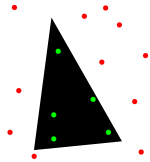
\includegraphics[width=0.4\textwidth]{se.png}
\caption{}
\end{figure} 
\subsection{Topology}
Although topology is the field of mathematics that formalizes and generalizes the intuitive notion of "continuous deformation" of objects, it gives rise to many discrete topics; this can be attributed in part to the focus on topological invariants, which themselves usually take discrete values. See combinatorial topology, topological graph theory, topological combinatorics, computational topology, discrete topological space, finite topological space, topology (chemistry). 
\subsection{Operations research}
Operations research provides techniques for solving practical problems in engineering, business, and other fields — problems such as allocating resources to maximize profit, and scheduling project activities to minimize risk. Operations research techniques include linear programming and other areas of optimization, queuing theory, scheduling theory, and network theory. Operations research also includes continuous topics such as continuous-time Markov process, continuous-time martingales, process optimization, and continuous and hybrid control theory.
\newpage
\begin{figure}[h]
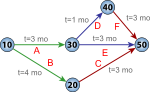
\includegraphics[width=0.4\textwidth]{sf.png}
\caption{Topology}
\end{figure} 
\subsection{Game theory, decision theory, utility theory, social choice theory}
Decision theory is concerned with identifying the values, uncertainties and other issues relevant in a given decision, its rationality, and the resulting optimal decision.

Utility theory is about measures of the relative economic satisfaction from, or desirability of, consumption of various goods and services.

Social choice theory is about voting. A more puzzle-based approach to voting is ballot theory.

Game theory deals with situations where success depends on the choices of others, which makes choosing the best course of action more complex. There are even continuous games, see differential game. Topics include auction theory and fair division. 
\subsection{Discretization} 
Discretization concerns the process of transferring continuous models and equations into discrete counterparts, often for the purposes of making calculations easier by using approximations. Numerical analysis provides an important example.
\subsection{Discrete analogues of continuous mathematics}
There are many concepts in continuous mathematics which have discrete versions, such as discrete calculus, discrete probability distributions, discrete Fourier transforms, discrete geometry, discrete logarithms, discrete differential geometry, discrete exterior calculus, discrete Morse theory, difference equations, discrete dynamical systems, and discrete vector measures.

In applied mathematics, discrete modeling is the discrete analogue of continuous modeling. In discrete modeling, discrete formula are fit to data. A common method in this form of modeling is to use recurrence relation.

In algebraic geometry, the concept of a curve can be extended to discrete geometries by taking the spectra of polynomial rings over finite fields to be models of the affine spaces over that field, and letting sub-varieties or spectra of other rings provide the curves that lie in that space. Although the space in which the curves appear has a finite number of points, the curves are not so much sets of points as analogues of curves in continuous settings.  Algebraic varieties also have a well-defined notion of tangent space called the Zariski tangent space, making many features of calculus applicable even in finite settings.  
\subsection{Hybrid discrete and continuous mathematics}
The time scale calculus is a unification of the theory of difference equations with that of differential equations, which has applications to fields requiring simultaneous modeling of discrete and continuous data. Another way of modeling such a situation is the notion of hybrid dynamical systems. 
\section{Outline of discrete mathematics}
Discrete mathematics is the study of mathematical structures that are fundamentally discrete rather than continuous. In contrast to real numbers that have the property of varying "smoothly", the objects studied in discrete mathematics – such as integers, graphs, and statements in logic – do not vary smoothly in this way, but have distinct, separated values.Discrete mathematics therefore excludes topics in "continuous mathematics" such as calculus and analysis.

Included below are many of the standard terms used routinely in university-level courses and in research papers. This is not, however, intended as a complete list of mathematical terms; just a selection of typical terms of art that may be encountered. 
\subsection{Subjects in discrete mathematics}
Information theory involves the quantification of information. Closely related is coding theory which is used to design efficient and reliable data transmission and storage methods. Information theory also includes continuous topics such as: analog signals, analog coding, analog encryption. 
\subsubsection{Logic}
The concepts of logical form and argument are central to logic. An argument is constructed by applying one of the forms of the different types of logical reasoning: deductive, inductive, abductive. In deduction, the validity of an argument is determined solely by its logical form, not its content, while the soundness requires both validity and that all the given premises are actually true.Completeness, consistency, decidability, and expressivity, are further fundamental concepts in logic. The categorization of the logical systems and of their properties has led to the emergence of a metatheory of logic known as metalogic.

    Informal logic is the study of natural language arguments. The study of fallacies is an important branch of informal logic. Since much informal argument is not strictly speaking deductive, on some conceptions of logic, informal logic is not logic at all. See § Rival conceptions below.
    Formal logic is the study of inference with purely formal content. An inference possesses a purely formal content if it can be expressed as a particular application of a wholly abstract rule, that is, a rule that is not about any particular thing or property. Traditional syllogistic logic, also known as term logic, and modern symbolic logic, the study of symbolic abstractions that capture the formal features of logical inference,are examples of formal logic. Symbolic logic is often divided into two main branches: propositional logic and predicate logic. The works of Aristotle contain the earliest known formal study of the syllogism. Modern formal logic follows and expands on Aristotle.In many definitions of logic, logical inference and inference with purely formal content are the same. This does not render the notion of informal logic vacuous, because no formal logic captures all of the nuances of natural language.
    Mathematical logic is an extension of symbolic logic into other areas, in particular to the study of model theory, proof theory, set theory, and computability theory.
However, agreement on what logic actually is has remained elusive, although the field of universal logic has studied the common structure of logic.
\section{Discrete mathematical disciplines}
For further reading in discrete mathematics, beyond a basic level, see these pages. Many of these disciplines are closely related to computer science.
\subsection{Automata theory}
Automata theory is the study of abstract machines and automata, as well as the computational problems that can be solved using them. It is a theory in theoretical computer science and discrete mathematics (a subject of study in both mathematics and computer science). The word automata (the plural of automaton) comes from the Greek word αὐτόματα, which means "self-making".

The figure at right illustrates a finite-state machine, which belongs to a well-known type of automaton. This automaton consists of states (represented in the figure by circles) and transitions (represented by arrows). As the automaton sees a symbol of input, it makes a transition (or jump) to another state, according to its transition function, which takes the current state and the recent symbol as its inputs.

Automata theory is closely related to formal language theory. An automaton is a finite representation of a formal language that may be an infinite set. Automata are often classified by the class of formal languages they can recognize, typically illustrated by the Chomsky hierarchy, which describes the relations between various languages and kinds of formalized logics.

Automata play a major role in theory of computation, compiler construction, artificial intelligence, parsing and formal verification.
\begin{figure}[h]
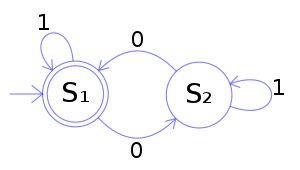
\includegraphics[width=0.4\textwidth]{sj.png}
\caption{Automata theory}
\end{figure}
\subsection{Coding theory} 
Coding theory is the study of the properties of codes and their respective fitness for specific applications. Codes are used for data compression, cryptography, error detection and correction, data transmission and data storage. Codes are studied by various scientific disciplines—such as information theory, electrical engineering, mathematics, linguistics, and computer science—for the purpose of designing efficient and reliable data transmission methods. This typically involves the removal of redundancy and the correction or detection of errors in the transmitted data.

There are four types of coding:[1]

    Data compression (or source coding)
    Error control (or channel coding)
    Cryptographic coding
    Line coding

Data compression attempts to remove redundancy from the data from a source in order to transmit it more efficiently. For example, Zip data compression makes data files smaller, for purposes such as to reduce Internet traffic. Data compression and error correction may be studied in combination.

Error correction adds extra data bits to make the transmission of data more robust to disturbances present on the transmission channel. The ordinary user may not be aware of many applications using error correction. A typical music CD uses the Reed-Solomon code to correct for scratches and dust. In this application the transmission channel is the CD itself. Cell phones also use coding techniques to correct for the fading and noise of high frequency radio transmission. Data modems, telephone transmissions, and the NASA Deep Space Network all employ channel coding techniques to get the bits through, for example the turbo code and LDPC code.
\begin{figure}[h]
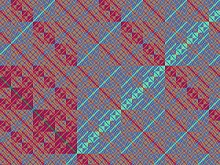
\includegraphics[width=0.2\textwidth]{sk.jpg}
\caption{A two-dimensional visualisation of the Hamming distance, a critical measure in coding theory}
\end{figure} 
\subsection{Discrete geometry}
Discrete geometry and combinatorial geometry are branches of geometry that study combinatorial properties and constructive methods of discrete geometric objects. Most questions in discrete geometry involve finite or discrete sets of basic geometric objects, such as points, lines, planes, circles, spheres, polygons, and so forth. The subject focuses on the combinatorial properties of these objects, such as how they intersect one another, or how they may be arranged to cover a larger object.

Discrete geometry has a large overlap with convex geometry and computational geometry, and is closely related to subjects such as finite geometry, combinatorial optimization, digital geometry, discrete differential geometry, geometric graph theory, toric geometry, and combinatorial topology. 
\begin{figure}[h]
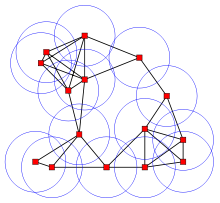
\includegraphics[width=0.4\textwidth]{sl.png}
\caption{A collection of circles and the corresponding unit disk graph}
\end{figure}
\subsection{Discrete Optimization}
Mathematical optimization (alternatively spelled optimisation) or mathematical programming is the selection of a best element (with regard to some criterion) from some set of available alternatives.[1] Optimization problems of sorts arise in all quantitative disciplines from computer science and engineering to operations research and economics, and the development of solution methods has been of interest in mathematics for centuries.[2]

In the simplest case, an optimization problem consists of maximizing or minimizing a real function by systematically choosing input values from within an allowed set and computing the value of the function. The generalization of optimization theory and techniques to other formulations constitutes a large area of applied mathematics. More generally, optimization includes finding "best available" values of some objective function given a defined domain (or input), including a variety of different types of objective functions and different types of domains.
\begin{figure}[h]
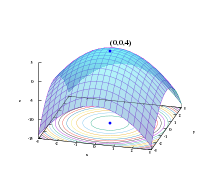
\includegraphics[width=0.4\textwidth]{sm.png}
\caption{Graph of a paraboloid given by z = f(x, y) = −(x² + y²) + 4. The global maximum at (x, y, z) = (0, 0, 4) is indicated by a blue dot.}
\end{figure}  
\section{Concepts in discrete mathematics}
\subsection{Set (mathematics)}
This article is about what mathematicians call "intuitive" or "naive" set theory. For a more detailed account, see Naive set theory. For a rigorous modern axiomatic treatment of sets, see Set theory.
In mathematics, a set is a well-defined collection of distinct objects, considered as an object in its own right.For example, the numbers 2, 4, and 6 are distinct objects when considered separately, but when they are considered collectively they form a single set of size three, written {2, 4, 6}. The concept of a set is one of the most fundamental in mathematics. Developed at the end of the 19th century, set theory is now a ubiquitous part of mathematics, and can be used as a foundation from which nearly all of mathematics can be derived.
\begin{figure}[h]
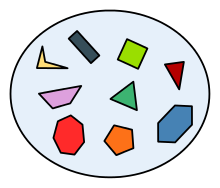
\includegraphics[width=0.4\textwidth]{sn.png}
\caption{A set of polygons in an Euler diagram}
\end{figure}
\subsection{Venn diagram}
A Venn diagram (also called primary diagram, set diagram or logic diagram) is a diagram that shows all possible logical relations between a finite collection of different sets. These diagrams depict elements as points in the plane, and sets as regions inside closed curves. A Venn diagram consists of multiple overlapping closed curves, usually circles, each representing a set. The points inside a curve labelled S represent elements of the set S, while points outside the boundary represent elements not in the set S. This lends to easily read visualizations; for example, the set of all elements that are members of both sets S and T, S ∩ T, is represented visually by the area of overlap of the regions S and T. In Venn diagrams the curves are overlapped in every possible way, showing all possible relations between the sets. They are thus a special case of Euler diagrams, which do not necessarily show all relations. Venn diagrams were conceived around 1880 by John Venn. They are used to teach elementary set theory, as well as illustrate simple set relationships in probability, logic, statistics, linguistics, and computer science.

A Venn diagram in which the area of each shape is proportional to the number of elements it contains is called an area-proportional or scaled Venn diagram. 
 \begin{figure}[h]
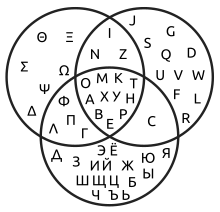
\includegraphics[width=0.4\textwidth]{so.png}
\caption{Venn diagram showing the uppercase glyphs shared by the Greek, Latin, and Cyrillic alphabets}
\end{figure}
\section{Elementary algebra}
Elementary algebra encompasses some of the basic concepts of algebra, one of the main branches of mathematics. It is typically taught to secondary school students and builds on their understanding of arithmetic. Whereas arithmetic deals with specified numbers,[1] algebra introduces quantities without fixed values, known as variables.[2] This use of variables entails a use of algebraic notation and an understanding of the general rules of the operators introduced in arithmetic. Unlike abstract algebra, elementary algebra is not concerned with algebraic structures outside the realm of real and complex numbers.

The use of variables to denote quantities allows general relationships between quantities to be formally and concisely expressed, and thus enables solving a broader scope of problems. Many quantitative relationships in science and mathematics are expressed as algebraic equations. 
\begin{figure}[h]
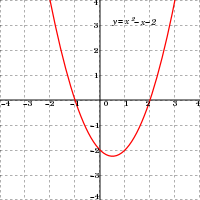
\includegraphics[width=0.4\textwidth]{sp.png}
\caption{Two-dimensional plot (red curve) of the algebraic equation  }
\end{figure}
\section{Mathematical relations}
\subsection{Special types of binary relations}
Some important types of binary relations R over two sets X and Y are listed below.

Uniqueness properties:

    Injective (also called left-unique[12]): for all x and z in X and y in Y, if xRy and zRy then x = z. For example, the green relation in the diagram is injective, but the red relation is not, as, e.g., it relates both −5 and 5 to 25.
    Functional (also called right-unique[12], right-definite[13] or univalent[14]): for all x in X, and y and z in Y, if xRy and xRz then y = z. Such a relation is called a partial function. Both relations in the picture are functional. An example of a non-functional relation can be obtained by rotating the red graph clockwise by 90 degrees, i.e. by considering the relation x = y2 which, e.g., relates 25 to both −5 and 5.
    One-to-one (also written 1-to-1): injective and functional. The green relation is one-to-one, but the red is not.

Totality properties (only definable if the sets of departure X resp. destination Y are specified):

    Left-total:[12] for all x in X there exists a y in Y such that xRy; such an R is also called a multivalued function by some authors.[citation needed] This property, although also referred to as total by some authors,[citation needed] is different from the definition of total in the section Properties. Both relations in the picture are left-total. The relation x = y2, obtained from the above rotation, is not left-total, as, for example, it doesn't relate −14 to any real number.
    Surjective (also called right-total[12] or onto): for all y in Y, there exists an x in X such that xRy. The green relation is surjective, but the red relation is not, as, for example, it doesn't relate any real number to −14.

Uniqueness and totality properties:

    A function: a relation that is functional and left-total. Both the green and the red relation are functions.
    An injective function or injection: a relation that is injective, functional, and left-total.
    A surjective function or surjection: a relation that is functional, left-total, and right-total.
    A bijection: a function that is surjective one-to-one (or surjective injective) is said to be bijective, also known as one-to-one correspondence.[15] The green relation is bijective, but the red is not. 
\subsection{Matrix representation}
 Binary relations over two sets X and Y can be represented algebraically by matrices indexed by X and Y with entries in the Boolean semiring (addition corresponds to OR and multiplication to AND), matrix addition corresponds to union of relations, matrix multiplication corresponds to composition of relations (of a relation over X and Y and a relation over Y and Z),the Hadamard product corresponds to intersection of relations, the zero matrix corresponds to the empty relation, and the matrix of ones corresponds to the universal relation. If X equals Y then the endorelations form a matrix semiring (indeed, a matrix semialgebra over the Boolean semiring), and the identity matrix corresponds to the identity relation. 
 \subsection{Equivalence relation}
 This article is about the mathematical concept. For the patent doctrine, see Doctrine of equivalents.
"Equivalency" redirects here. For other uses, see Equivalence.
This article is about the mathematical concept. For the patent doctrine, see Doctrine of equivalents.
"Equivalency" redirects here. For other uses, see Equivalence.
\begin{figure}[h]
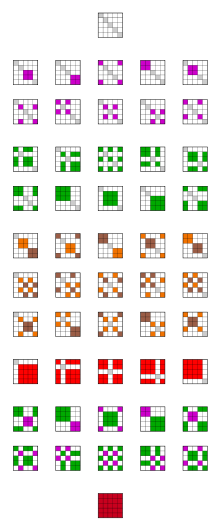
\includegraphics[width=0.2\textwidth]{sq.png}
\caption{Equivalence relation}
\end{figure}
\newpage
\section{Propositional logic} 
\subsection{Logical connective}
In logic, a logical connective (also called a logical operator, sentential connective, or sentential operator) is a symbol or word used to connect two or more sentences (of either a formal or a natural language) in a grammatically valid way, such that the value of the compound sentence produced depends only on that of the original sentences and on the meaning of the connective.
\begin{figure}[h]
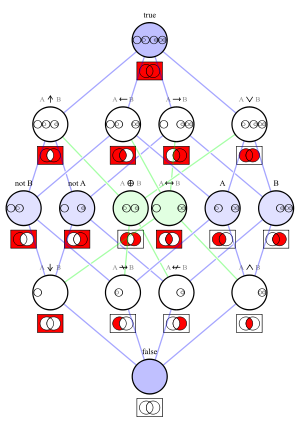
\includegraphics[width=0.2\textwidth]{smm.png}
\caption{Hasse diagram of logical connectives.}
\end{figure}
\subsection{Truth table}
A truth table is a mathematical table used in logic—specifically in connection with Boolean algebra, boolean functions, and propositional calculus—which sets out the functional values of logical expressions on each of their functional arguments, that is, for each combination of values taken by their logical variables (Enderton, 2001). In particular, truth tables can be used to show whether a propositional expression is true for all legitimate input values, that is, logically valid.

A truth table has one column for each input variable (for example, P and Q), and one final column showing all of the possible results of the logical operation that the table represents (for example, P XOR Q). Each row of the truth table contains one possible configuration of the input variables (for instance, P=true Q=false), and the result of the operation for those values. See the examples below for further clarification. Ludwig Wittgenstein is generally credited with inventing and popularizing the truth table in his Tractatus Logico-Philosophicus, which was completed in 1918 and published in 1921 Such a system was also independently proposed in 1921 by Emil Leon Post. An even earlier iteration of the truth table has also been found in unpublished manuscripts by Charles Sanders Peirce from 1893, antedating both publications by nearly 30 years.
The most common logical connectives are binary connectives (also called dyadic connectives) which join two sentences which can be thought of as the function's operands. Also commonly, negation is considered to be a unary connective.

Logical connectives along with quantifiers are the two main types of logical constants used in formal systems such as propositional logic and predicate logic. Semantics of a logical connective is often, but not always, presented as a truth function.

A logical connective is similar to but not equivalent to a conditional operator.
\subsubsection{Logical True}
The output value is always true, regardless of the input value of p.


\begin{center}
\begin{tabular}{ |c|c|} 
\hline
P&T \\ 
\hline
T&T \\ 
\hline
F&T \\ 
\hline
\end{tabular}
\end{center}
\subsubsection{Logical false}

 \begin{center}
\begin{tabular}{ |c|c|} 
\hline
P&F \\ 
\hline
T&F \\ 
\hline
F&F \\ 
\hline
\end{tabular}
\end{center}
\subsubsection{Logical identity}
Logical identity is an operation on one logical value p, for which the output value remains p.

The truth table for the logical identity operator is as follows:
Logical Identity 
 \begin{center}
\begin{tabular}{ |c|c|} 
\hline
P&P \\ 
\hline
T&T \\ 
\hline
F&F \\ 
\hline
\end{tabular}
\end{center}
\subsubsection{Logical negation}
Logical negation is an operation on one logical value, typically the value of a proposition, that produces a value of true if its operand is false and a value of false if its operand is true.

The truth table for NOT p (also written as ¬p, Np, Fpq, or ~p) is as follows: 
 \begin{center}
\begin{tabular}{ |c|c|} 
\hline
P&¬P \\ 
\hline
T&F \\ 
\hline
F&T \\ 
\hline
\end{tabular}
\end{center}
\subsection{De Morgan's laws}
In propositional logic and boolean algebra, De Morgan's laws[1][2][3] are a pair of transformation rules that are both valid rules of inference. They are named after Augustus De Morgan, a 19th-century British mathematician. The rules allow the expression of conjunctions and disjunctions purely in terms of each other via negation.

The rules can be expressed in English as:

    the negation of a disjunction is the conjunction of the negations; and
    the negation of a conjunction is the disjunction of the negations;

or

    the complement of the union of two sets is the same as the intersection of their complements; and
    the complement of the intersection of two sets is the same as the union of their complements.

or

    not (A or B) = not A and not B; and
    not (A and B) = not A or not B
\begin{figure}[h]
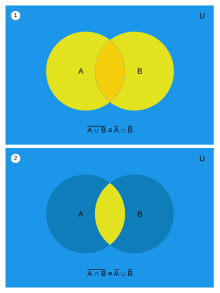
\includegraphics[width=0.4\textwidth]{ssm.png}
\caption{De Morgan's laws represented with Venn diagrams. In each case, the resultant set is the set of all points in any shade of blue.}
\end{figure}
\section{Importance of discrete mathematics}
Computer science is the study of problems, problem solving and the solutions that come out of the problem solving process, B. Miller and D. Ranum (2013). A computer scientist goal is to develop an algorithm, a step by step list of instructions in solving a problem. Algorithms are finite processes that if followed will solve the problem

Discrete mathematics is concerned with structures which take on a discrete value often infinite in nature. Just as the real-number system plays a crucial role in continuous mathematics, integers are the cornerstone in discrete mathematics. Discrete mathematics provides excellent modelling tools for analysing real-world phenomena that varies in one state or another and is a vital tool used in a wide range of applications, from computers to telephone call routing and from personnel assignments to genetics, E.R. Scheinerman (2000) cited in W. J. Rapaport 2013).

The difference between discrete mathematics and other disciplines is the basic foundation on proof as its modus operandi for determining truth, whereas science for example, relies on carefully analysed experience. According to J. Barwise and J. Etchemendy, (2000), a proof is any reasoned argument accepted as such by other mathematicians.

Discrete mathematics is the background behind many computer operations (A. Purkiss 2014, slide 2) and is therefore essential in computer science. According to the National Council of Teachers of Mathematics (2000), discrete mathematics is an essential part of the educational curriculum (Principles and Standards for School Mathematics, p. 31). K. H Rosen (2012) cites several important reasons for studying discrete mathematics including the ability to comprehend mathematical arguments. In addition he argues discrete mathematics is the gateway to advanced courses in mathematical sciences.

This essay will discuss the importance of discrete mathematics in computer science. Furthermore, it will attempt to provide an understanding of important related mathematical concepts and demonstrate with evidence based research why these concepts are essential in computer science. The essay will be divided into sections. Section one will define and discuss the importance of discrete mathematics. The second section will focus on and discuss discrete structures and relationships with objects. The set theory would be used as an example and will give a brief understanding of the concept. The third section will highlight the importance of mathematical reasoning. Finally, the essay will conclude with an overview of why discrete mathematics is essential in computer science.
Reference:\\
\url{<www.google.com>}

\end{document}